\documentclass[a4paper,12pt]{exam}
\usepackage{graphicx} % Required for inserting images
\usepackage[margin-1in]{geometry}
\setlength{\textheight}{23cm} 
\usepackage{amsmath}
\setlength{\parskip}{0pt}
\usepackage{setspace}
\usepackage{fancyhdr}
\usepackage{gvv-book}
\usepackage{gvv}
\usepackage{cite}
\usepackage{amsmath,amssymb,amsfonts,amsthm}
\usepackage{algorithmic}
\usepackage{graphicx}
\usepackage{textcomp}
\usepackage{xcolor}
\usepackage{txfonts}
\usepackage{listings}
\usepackage{enumitem}
\usepackage{mathtools}
\usepackage{gensymb}
\usepackage{comment}
\usepackage[breaklinks=true]{hyperref}
\usepackage{tkz-euclide} 
\usepackage{listings}
\usepackage{gvv}                                        
\def\inputGnumericTable{}                                 
\usepackage[latin1]{inputenc}                                
\usepackage{xcolor}                                            
\usepackage{array}                                            
\usepackage{longtable}                                       
\usepackage{calc}                                             
\usepackage{multirow}                                         
\usepackage{hhline}                                           
\usepackage{ifthen}                                           
\usepackage{lscape}
\usepackage{circuitikz}

\renewcommand{\thefigure}{\theenumi}
\renewcommand{\thetable}{\theenumi}
\setlength{\intextsep}{10pt} % Space between text and floats
\numberwithin{equation}{enumi}
\numberwithin{figure}{enumi}
\renewcommand{\thetable}{\theenumi}
\pagestyle{fancy}
\fancyhf{}
\fancyhead[L]{EE25BTECH11045}
\fancyhead[R]{Biomedical Engineering(BM)}

\graphicspath{ {./figs/} }

\begin{document}

\bibliographystyle{IEEEtran}
\vspace{-2cm}
\title{GATE 2024 BT24S3}
\author{EE25BTECH11045 - P.Navya Priya}

{\let\newpage\relax\maketitle}
\renewcommand{\thefigure}{\theenumi}
\renewcommand{\thetable}{\theenumi}

\vspace*{-1.5cm}
\begin{flushright}
\textbf{Biomedical Engineering(BM)}
\end{flushright}

\vspace{2cm}


\vspace{-1cm}
\noindent{\large \textbf{\underline{General Aptitude(GA)}}}
\vspace{0.75cm}

\vspace*{-0.5cm}
\noindent{\large\textbf{Q.1-Q.5 Carry ONE mark Each}}
\vspace{0.75cm}
\begin{enumerate}
\item If `$\longrightarrow$' denotes increasing order of intensity, then the meaning of the words [simmer $\longrightarrow$ seethe $\longrightarrow$ smolder] is analogous to [break $\longrightarrow$ raze$\longrightarrow$ \underline{\hspace{1cm}}].Which one of the options is appropriate to fill the blank?

\hfill{\brak{\text{GATE BM 2024}}}

\begin{multicols}{4}
\begin{enumerate}
\item obfuscate
\item obliterate
\item fracture
\item fissure
\end{enumerate}
\end{multicols}


\item In a  locality, the houses are numbered in the following way:\\[8pt] The house-numbers on one side of a road are consecutive odd integers starting from 301, while the house-numbers on the other side of the road are consecutive even 
 numbers starting from 302. The total number of houses is the same on both sides of the road.\\[8pt] If the difference of the sum of the house-numbers between the two sides of the road is 27, then the number of houses on each side of the road is 

\hfill{\brak{\text{GATE BM 2024}}}

\begin{multicols}{4}
\begin{enumerate}
\item 27
\item 52
\item 54
\item 26
\end{enumerate}
\end{multicols}

\item For positive integers $p$ and $q$, with $\frac{p}{q}\ne 1$, $\left(\frac{p}{q}\right)^{\frac{p}{q}}$ = $p^{\left(\frac{p}{q}-1\right)}$. Then,

\hfill{\brak{\text{GATE BM 2024}}}

\begin{multicols}{4}
\begin{enumerate}
\item $q^{p} = p^q$
\item $q^p = q^{2q}$
\item $\sqrt{q} = \sqrt{p}$
\item $\sqrt[p]{q} = \sqrt[q]{p}$
\end{enumerate}
\end{multicols}

\item Which  one of the given options is a possible value of $X$ in the following sequence?

\begin{align*}
3,\ 7,\ 15,\ X,\ 63,\ 127,\ 255
\end{align*}

\hfill{\brak{\text{GATE BM 2024}}}

\begin{multicols}{4}
\begin{enumerate}
\item 35
\item 40
\item 45
\item 31
\end{enumerate}
\end{multicols}

\item On a given day, how many times  will the second-hand and the minute-hand of a  clock cross each other during the clock time 12:05:00 hours to 12:55:00 hours?

\hfill{\brak{\text{GATE BM 2024}}}

\begin{multicols}{4}
\begin{enumerate}
\item 51
\item 49
\item 50
\item 55
\end{enumerate}
\end{multicols}

\textbf{Q.6-Q.10 Carry TWO marks Each}
\vspace{0.2cm}


\item In the given text, the blanks are numbered (i)-(iv). Select the best match for  all the blanks.\\
From the ancient Athenian arena to the modern Olympic  stadiums,  athletics{\underline{\hspace{0.5cm}(i)\hspace{0.5cm}}} the potential for a spectacle. The crowd {\underline{\hspace{0.5cm}(ii)\hspace{0.5cm}}}  
with bated breath as the Olympian artist twists his body, stretching the javelin behind him.Twelve strides in, he begins to cross-step. Six cross-steps {\underline{\hspace{0.5cm}(iii)\hspace{0.5cm}}} in an abrupt  stop on his left foot. As his body {\underline{\hspace{0.5cm}(iv)\hspace{0.5cm}}} like a door turning on a hinge, the  javelin is launched skyward at a precise angle. 

\hfill{\brak{\text{GATE BM 2024}}}

\begin{enumerate}

\item (i)hold\hspace{0.75cm}(ii)waits\hspace{0.75cm}(iii)culminates\hspace{0.75cm}(iv)pivot
\item (i)holds\hspace{0.75cm}(ii)wait\hspace{0.75cm}(iii)culminates\hspace{0.75cm}(iv)pivot
\item (i)hold\hspace{0.75cm}(ii)wait\hspace{0.75cm}(iii)culminate\hspace{0.75cm}(iv)pivots
\item (i)holds\hspace{0.75cm}(ii)waits\hspace{0.75cm}(iii)culminate\hspace{0.75cm}(iv)pivots
\end{enumerate}


\item Three distinct sets of indistinguishable twins are to be seated at a circular table that  has 8 identical chairs. Unique seating arrangements are defined by the relative  positions of the people.\\  How many unique seating arrangements are possible such that each person is sitting 
next to their twin?

\hfill{\brak{\text{GATE BM 2024}}}

\begin{multicols}{4}
\begin{enumerate}
    \item 12
    \item 14
    \item 10
    \item 28
\end{enumerate}
\end{multicols}

\item The chart given below compares the Installed Capacity (MW) of four power 
generation technologies, T1, T2, T3, and T4, and their Electricity Generation  
(MWh) in a time of 1000 hours (h). 

\begin{figure}[H]
\centering
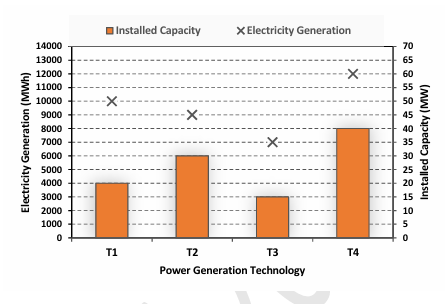
\includegraphics[width=1\columnwidth]{figs/Q8.png}
\label{fig:Q8.png}
\end{figure}


\hspace{0.75cm}The Capacity Factor of a power generation technology is:  \\


\begin{equation*}
\text{Capacity Factor} = \frac{\text{\large Electricity Generation (MWh)}}{\text{\large Installed Capacity (MW)} \times \text{1000 (h)}}
\end{equation*} 

\hfill{\brak{\text{GATE BM 2024}}}

\begin{multicols}{4}
\begin{enumerate}
 \item T1
\item T2
\item T3
\item T4
\end{enumerate} 
\end{multicols}

\item In the 4 × 4 array shown below, each cell of the first three columns has either a cross ($X$) or a number, as in the given rule. 

\begin{figure}[h]
\centering
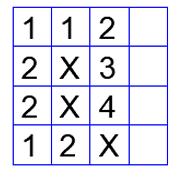
\includegraphics[width=0.25\columnwidth]{figs/Q9.png}
\label{fig:Q9.png}
\end{figure}

\textbf{Rule:} The number in a cell represents the count of crosses around its immediate neighboring cells (left, right, top, bottom, diagonals).\\ As per this rule, the \textbf{maximum} number of crosses possible in the empty column is 

\hfill{\brak{\text{GATE BM 2024}}}

\begin{multicols}{4}
\begin{enumerate}
    \item 0
    \item 1
    \item 2
    \item 3
\end{enumerate}
\end{multicols}

\item During a half-moon phase, the Earth-Moon-Sun form a right triangle. If the  Moon-Earth-Sun angle at this half-moon phase is measured to be 89.85°, the ratio  of the Earth-Sun and Earth-Moon distances is closest to

\hfill{\brak{\text{GATE BM 2024}}}

\begin{multicols}{4}
\begin{enumerate}
 \item 328
\item 382
\item 238
\item 283
\end{enumerate}
\end{multicols}

\textbf{Q.11 - Q.35 Carry ONE mark Each}
\vspace{0.25cm}

\item What is the value of the following complex line integral counter-clockwise? \\
\begin{align*}
\displaystyle\oint_{|\text{z}| = 3} \,\frac{8}{\text{z(z - 2)(z - 4)}} \, dz
\end{align*}

\hfill{\brak{\text{GATE BM 2024}}}

\begin{multicols}{4}
\begin{enumerate}
 \item $+j2\pi$
\item $-j2\pi$
\item $-j10\pi$
\item $+j10\pi$
\end{enumerate}  
\end{multicols}


\item To solve the equation $x = 2 \cos x$ using Newton-Raphson's method, which one of the following iterations should be used? 

\hfill{\brak{\text{GATE BM 2024}}}

\begin{enumerate}
\item  $x_{n+1} = x_n - \frac{x_n - 2\cos x_n}{1 + 2\sin x_n}$
\vspace{0.5cm}
\item  $x_{n+1} = x_n + \frac{x_n - 2\cos x_n}{1 + 2\sin x_n}$
\vspace{0.5cm}
\item  $x_{n+1} = x_n + \frac{1 + 2\sin x_n}{x_n - 2\cos x_n}$
\vspace{0.5cm}
\item  $x_{n+1} = x_n - \frac{1 + 2\sin x_n}{x_n - 2\cos x_n}$
\end{enumerate}  

\vspace{0.25cm}

\item During the repolarization phase of a neuron, the cell is brought back to the resting potential by the action of a Sodium-Potassium pump. Which one of the following  statements is \textbf{TRUE} for the active transport of Na+ and K+ ions through the cell membrane?

\hfill{\brak{\text{GATE BM 2024}}}

\begin{enumerate}
 \item For every 3 Na+ transported out of the cell 2 K+ is transported into the cell.
\item For every 3 $\text{Na}^+$ transported into the cell 2 $\text{K}^+$ is transported out of the cell.
\item For every 2 $\text{Na}^+$ transported out of the cell 3 $\text{K}^+$ is transported into the cell. 
\item The ratio of $\text{Na}^+$ and $\text{K}^+$ transport is always equal to one.
\end{enumerate}  

\item The cardiac rhythm in a healthy human heart originates from \underline{\hspace{1cm}}.

\hfill{\brak{\text{GATE BM 2024}}}

\begin{enumerate}
\item Sinu-atrial node (SA) 
\item Atrio-ventricular node (AV) 
\item Aorta 
\item Right atria 
\end{enumerate} 

\item Which one of the following events is \text{NOT} typically encountered in diagnostic X-ray projection radiography?

\hfill{\brak{\text{GATE BM 2024}}}

\begin{enumerate}
 \item Pair production 
\item Photoelectric absorption 
\vspace{0.25cm}
\item Compton scattering 
\item Characteristic radiation 
\end{enumerate}  

\item Which of the following statements is \textbf{TRUE} for a PET imaging system?    

\hfill{\brak{\text{GATE BM 2024}}}

\begin{enumerate}
 \item Two coincident photons of 511 keV energy are detected $180^\circ$ apart. 
\item Photons of 51.1 keV energy are detected $360^\circ$ around the body.  
\item Photons of energy 511 keV are detected $360^\circ$ around the body.
\item Coincident photons with 51.1 keV energy are detected $180^\circ$ apart. 
\end{enumerate}  

\item Consider the following layers: subcutaneous fat, viable epidermis, stratum 
corneum, and dermis. Which one of the following represents the correct sequence  of the layers from skin surface to within?

\hfill{\brak{\text{GATE BM 2024}}}

\begin{enumerate}
 \item Dermis, subcutaneous fat, viable epidermis, stratum corneum 
\item Dermis, viable epidermis, subcutaneous fat, stratum corneum
\item Stratum corneum, viable epidermis, dermis, subcutaneous fat 
\item Viable epidermis, stratum corneum, dermis, subcutaneous fat 
\end{enumerate}  

\item Bioglass 45S5 has a composition of \underline{\hspace{1.5cm}}.

\hfill{\brak{\text{GATE BM 2024}}}

\begin{enumerate}
 \item wt\% $SiO_2$ and 5:1 molar ratio of Calcium to Phosphorus.
\item 45 wt\% Hydroxyapatite and 5 wt\% $SiO_2$. 
\item 45 wt\% Hydroxyapatite and 5:1 molar ratio of CaO and $Ca3(PO_4)_2$.
\item 45 wt\% $SiO_2$ and 5 wt\% Hydroxyapatite. 
\end{enumerate}  

\item Marcophages that are resident in the liver are

\hfill{\brak{\text{GATE BM 2024}}}

\begin{enumerate}
    \item Histiocyte cells
    \item Langerhans cells
    \item Kupffer cells
    \item Fibroblast cells
\end{enumerate}

\item Which one of the following drug release kinetic curves will be ideal for developing an implantable slow-release drug delivery device?

\hfill{\brak{\text{GATE BM 2024}}}

\begin{figure}[H]
\begin{flushleft}
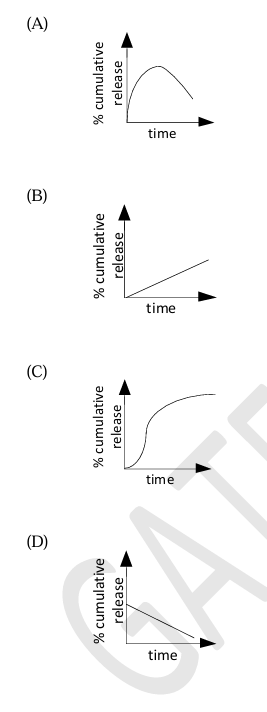
\includegraphics[width=0.2\columnwidth]{figs/Q20.png}
\label{fig:Q20.png}
\end{flushleft}
\end{figure}

\item The Bode plot of a $2^{\text{nd}}$ order low pass filter is shown in the figure below. What is the frequency at which the attenuation is 80 dB?

\begin{figure}[H]
\centering
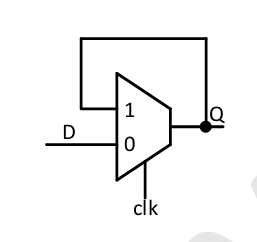
\includegraphics[width=0.25\textwidth]{figs/Q21.png}
\label{fig:Q21.png}
\end{figure}

\hfill{\brak{\text{GATE BM 2024}}}

\begin{enumerate}
 \item Negative level triggered D-latch 
\item Positive level triggered D-latch 
\item Negative edge triggered D-flip-flop
\item Positive edge triggered D-flip-flop  
\end{enumerate}  

\item The Fourier transform of $e^{-| 2\text{t} |}$ is \underline{\hspace{1cm}}.

\hfill{\brak{\text{GATE BM 2024}}}

\begin{multicols}{4}
\begin{enumerate}
\item $\frac{4}{4 - \omega^2}$
\item$\frac{4}{4 + \omega^2}$
\item $\frac{2}{2 + \omega}$
\item $\frac{2}{2 + \omega}$
\end{enumerate} 
\end{multicols}

\item The Bode plot of a $2^{\text{nd}}$ order low pass filter is shown in the figure below. What is the frequency at which the attenuation is 80 dB?

\begin{figure}[H]
\centering
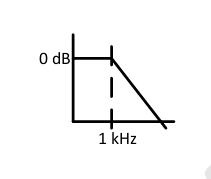
\includegraphics[width=0.3\columnwidth]{figs/Q23.png}
\label{fig:Q23.png}
\end{figure}

\hfill{\brak{\text{GATE BM 2024}}}

\begin{enumerate}
\item 10 kHz
\item 10 MHz
\item 100 kHz 
\item 100 MHz
\end{enumerate}  

\item The input $x(t)$ and the output $y(t)$ of a linear time invariant system are related as 
follows: \\[3pt]
\begin{equation*}
y(t) + \frac{dy(t)}{dt} 0.5\frac{d^2y(t)}{dt^2} = x(t) + 0.1\frac{dx(t)}{dt} 
\end{equation*}
What is the Laplace transform of the impulse response of the system? 

\hfill{\brak{\text{GATE BM 2024}}}

\begin{enumerate}
\item $\frac{0.5s^2 + s + 1}{0.1s + 1}$
\vspace{0.25cm}
\item $\frac{0.1s + 1}{0.5s^2 + s + 1}$
\vspace{0.25cm}
\item $\frac{0.1s + s^2}{s^2 + s + 0.5}$
\vspace{0.25cm}
\item $\frac{s^2 + s + 0.5}{0.1s^2 + s}$
\end{enumerate}  

\item Match the different chambers/locations of a healthy human heart in Column-1 to the ranges of \textbf{diastolic} pressures in Column-2.

\begin{table}[H]
\begin{center}
\def\arraystretch{2}
\begin{tabular}{|m{5cm}|m{5cm}|}
\hline
\text{\hspace{1cm}Column-1} & \text{\hspace{1cm}Column-2}\\ \hline
(P) \quad Arterial & (I) \quad 2-6 mm Hg \\ \hline
(Q)\quad Pulmonary artery & (II) \quad 8-12 mm Hg \\ \hline
(R) \quad Right ventricle & (III) \quad 60-80 mm Hg \\ \hline
\end{tabular}
\end{center}
\end{table}
\hfill{\brak{\text{GATE BM 2024}}}


\begin{enumerate}
\item (P) $-$ (II), (Q) $-$  (III), (R) $-$  (I)
\item (P) $-$  (II), (Q) $-$  (I), (R) $-$  (III) 
\item (P) $-$  (III), (Q) $-$  (II), (R) $-$  (I) 
\item (P) $-$  (III), (Q) $-$  (I), (R) $-$  (II)
\end{enumerate}  

\item Which of the following is/are \textbf{NOT TRUE} about photoreceptor cells in a healthy  human retina? 

\hfill{\brak{\text{GATE BM 2024}}}

\begin{enumerate}
\item The distribution of rod and cone cells is uniform all over the retina. 
\item The number of rods are higher than the number of cones in the retina.
\item Rods contain photopsin pigment. 
\item Cones are responsible for colour vision in bright light.
\end{enumerate}  

\item A monochromatic beam of $\gamma$-ray photons is incident on a homogenous tissue. Which  of the following relationships hold(s) \textbf{TRUE} for the half-value layer thickness? 

\hfill{\brak{\text{GATE BM 2024}}}

\begin{enumerate}
\item The first half-value layer is thicker than the second half-value layer.
\item The second half-value layer is thicker than the first half-value layer. 
\item All the half-value layers have equal thickness.
\item The ratio of thickness of the first and second half-value layers change based on the   intensity of the incident beam.
\end{enumerate}  

\item A group of four people were residing together when a new virus was detected. If  the probability of each person being infected is 0.1, then the probability that at least two of them are infected is \underline{\hspace{0.75cm}}. Give your answer rounded off to 3 decimal places. 

\hfill{\brak{\text{GATE BM 2024}}}

\item A random noise signal with Gaussian distribution has a mean of zero and a standard  deviation of 1 mV. The probability that an instantaneous measurement of this signal is greater than 2 mV or lesser than -2 mV is \underline{\hspace{1cm}}. Give your answer as a percentage rounded off to the nearest integer.

\hfill{\brak{\text{GATE BM 2024}}}

\item The trigonometric Fourier series expansion of the periodic function in the figure has coefficients {$a_n$} and {$b_n$} for cosine and sine terms, respectively. The value of  
$a_1/a_3$ is \underline{\hspace{1.2cm}}. Give your answer rounded off to 1 decimal place.  

\begin{figure}[H]
\hspace{1.5cm}
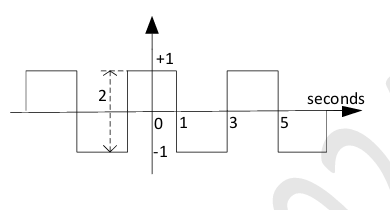
\includegraphics[width=0.5\columwidth]{figs/Q30.png}
\label{fig:Q30.png}
\end{figure}

\item A cylindrical engineered tissue was developed with a diameter of 2 cm, height of 3cm and Young’s modulus of 20 MPa. If an axial tensile force of 10 N is applied, the percentage change in the height of the tissue is \underline{\hspace{1cm}}\%. Give your answer rounded off to 2 decimal places.

\hfill{\brak{\text{GATE BM 2024}}}

\item The measured current through a device is 5 A, the voltage measured across the  device is 20 V. The ammeter and the voltmeter used for these measurements have  a measurement uncertainty of 1\% each. The maximum error in estimation of   impedance of the device is \underline{\hspace{1.5cm}} m$\Omega$. Give your answer rounded to the nearest 
integer. 

\hfill{\brak{\text{GATE BM 2024}}}

\item The Larmor frequency of a Na nucleus when placed in a magnetic field strength of 3 T is \underline{\hspace{2cm}}.(The gyromagnetic ratio of Na is given as $\gamma$ = 11.26 MHz/T.)   Give your answer in MHz rounded off to the nearest integer.

\hfill{\brak{\text{GATE BM 2024}}}

\item A Doppler ultrasound transducer operating at 5 MHz gave maximum output  frequency shift of 3 kHz. The velocity of sound in blood is 1500 m/s. If the probe was held at an angle of $45^\circ$ to the direction of blood flow, the maximum velocity of  blood flow through the artery is \underline{\hspace{0.75cm}} m/s. (Give your answer rounded off to two 
decimal places.)


\begin{figure}[h]
\hspace{5cm}
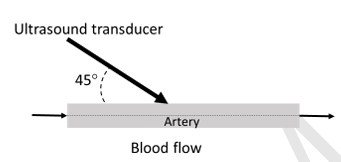
\includegraphics[width=0.5\textwidth]{figs/Q34.png}
\label{fig:Q34.png}
\end{figure}
\hfill(BM 2024)
\vspace{3cm}

\item The wavelength of the peak emission from a human body at a temperature of $37^\circ$  due to black-body radiation is \underline{\hspace{1cm}} $\mu$m. The value of Wien’s displacement  constant is $2.898 \times 10^{-3}$ m K. (Give your answer rounded off to 2 decimal places.)

\hfill{\brak{\text{GATE BM 2024}}}

\textbf{Q.36 - Q.65 Carry TWO marks each}

\vspace{0.25cm}

\item If $A = \begin{pmatrix} 1 & -1 \\ 2 & -2 \end{pmatrix}$, the eigenvalues of $A$ are \underline{\hspace{2cm}}.

\hfill{\brak{\text{GATE BM 2024}}}

\begin{multicols}{4}
\begin{enumerate}
\item $-1$ and 0
\item $-1$ and $+1$
\item $-1$ and $-1$
\item $+1$ and 0
\end{enumerate}
\end{multicols}

\item Consider a system of the following two partial differential equations: \\

\begin{equation*}
\frac{\partial\alpha}{\partial x} = -2\frac{\partial\beta}{\partial t}  
\end{equation*}

\vspace{8pt}

\begin{equation*}
\frac{\partial\beta}{\partial x} = -2\frac{\partial\alpha}{\partial t}
\end{equation*}
Which one of the following choices is a possible solution for the system? 

\hfill{\brak{\text{GATE BM 2024}}}

\begin{enumerate}
\item $\alpha(t, x) = (x -t)^2 + (x + t)^2 \, \text{and} \, \beta(t, x) = (x - t)^2 - (x + t)^2$.
\vspace{0.25cm}
\item $\alpha(t, x) = (x - 2t)^2 + (x + 2t)^2 \, \text{and} \,  \beta(t, x) = (x - 2t)^2 - (x + 2t)^2$.
\vspace{0.25cm}
\item $\alpha(t, x) = \left(x - \frac{t}{2}\right)^2 + \left(x + \frac{t}{2}\right)^2 \, \text{and} \, \beta(t, x) = \left(x - \frac{t}{2}\right)^2 - \left(x + \frac{t}{2}\right)^2$
\vspace{0.25cm}
\item $\alpha(t, x) = \left(x - \frac{t}{2}\right)^2 + 2\left(x + \frac{t}{2}\right)^2 \, \text{and} \, \beta(t, x) = 2\left(x - \frac{t}{2}\right)^2 - \left(x + \frac{t}{2}\right)^2$
\vspace{0.5cm}
\end{enumerate}  

\item The end-diastolic ventricular volume is found to be 125 mL and the end-systolic  ventricular volume is found to be 50 mL. If the heart rate is 65 beats/minute, what is the cardiac output in liters per minute? (Rounded off to 2 decimal places.)

\hfill{\brak{\text{GATE BM 2024}}}

\begin{multicols}{4}
\begin{enumerate}
\item 3.25
\vspace{0.5cm}
\item 4.88
\vspace{0.5cm}
\item 5.20
\vspace{0.5cm}
\item 3.00
\vspace{0.5cm}
\end{enumerate} 
\end{multicols}

\item Which of the following waveforms represents the output $\textbf{V}_o$ of the circuit given  below? The Zener diode used has a Zener breakdown voltage of 1 V and can be  assumed ideal while in forward bias.

\hfill{\brak{\text{GATE BM 2024}}}

\begin{figure}[H]
\hspace{0.75cm}
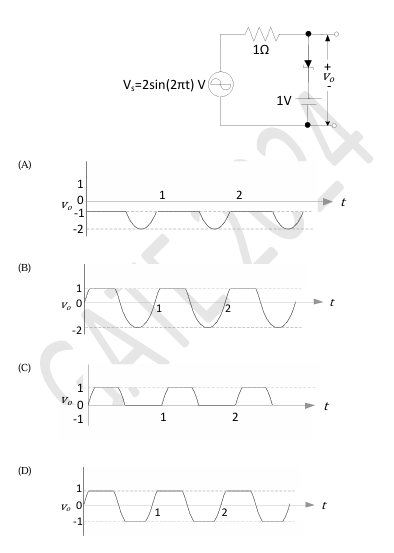
\includegraphics[width=0.5\columnwidth]{figs/Q39.png}
\label{fig:Q39.png}
\end{figure}

\item In magnetic resonance imaging (MRI), pulse repetition time (T R), time to echo (T E), $T_1$ relaxation time, $T_2$ relaxation time are some of the important pulse sequence design
parameters. Which one of the following specifications is used for proton density weighted imaging? 

\hfill{\brak{\text{GATE BM 2024}}}

\begin{enumerate}
\item $TR >> T_1 , TE << T_2$
\item $TR >> T_1 , TE >> T_2$
\item $TR << T_1 , TE << T_2$
\item $TR << T_1 , TE >> T_2$
\end{enumerate}  

\item An orthopaedic implant when monitored over 6 months showed the following normalized curves for polymer molecular weight (MW), mass of implant and mechanical strength. Among the choices, what is the most probable reason for the observed changes? 

\begin{figure}[h]
\centering
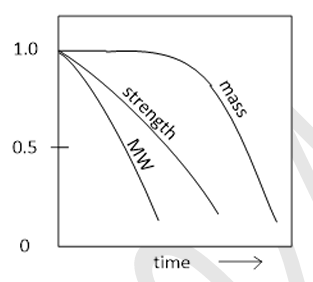
\includegraphics[width=0.5\columnwidth]{figs/Q41.png}
\label{fig:Q41.png}
\end{figure}

\begin{enumerate}
\item Bulk erosion
\item Surface erosion
\item Bulk initially followed by surface erosion
\item No erosion but mechanical breakage due to injury
\end{enumerate}  

\item In an attempt to integrate engineered tissue with native tissue, three samples of  engineered tissue, X, Y, Z, with identical material properties, were co-cultured adjacent to three different native tissues (bone, cartilage and liver). The adhesive \\ strengths of X, Y, Z were observed after 8 weeks as follows. \\[8pt] 
 Adhesive strength for X = 150 kPa, Y= 250 kPa, Z= 350 kPa \\[8pt]   Match the native tissue that were used to co-culture X, Y and Z from the following. \\[8pt]  I: Liver Tissue \\[8pt]  II: Articular Cartilage \\[8pt] III: Devitalized Bone

\hfill{\brak{\text{GATE BM 2024}}}

\begin{enumerate}
\item X with I,  Y with II and Z with III  
\item X with II,  Y with III and Z with I 
\item X with I,  Y with III and Z with II 
\item X with III,  Y with II and Z with I  
\end{enumerate}  

\item In a catheter-sensor system to measure blood pressure (P) as shown in the below figure, the liquid resistance ($R_L$) of the catheter is due to friction between shearing molecules flowing through the catheter. Which of the following is \textbf{TRUE} for $R_L$ if only the radius  of the catheter is doubled.Assume that the pressure difference across the catheter 
segment is fixed.

\begin{figure}[H]
\centering
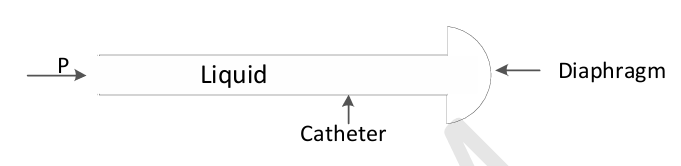
\includegraphics[width=0.6\columnwidth]{figs/Q43.png}
\label{fig:Q43.png}
\end{figure}

\hfill{\brak{\text{GATE BM 2024}}}

\begin{enumerate}
\item $R_L$  will decrease by 16 times
\item $R_L$  will decrease by 8 times
\item $R_L$  will decrease by 4 times
\item $R_L$  will decrease by 2 times
\end{enumerate}  

\item What is the value of the following integral using the residue integration method?

\begin{equation*}
\displaystyle\int\limits_{-\infty}^\infty\frac{dx}{1 + x^4}
\end{equation*}

\hfill{\brak{\text{GATE BM 2024}}}

\begin{multicols}{4}
\begin{enumerate}
\item $\frac{\pi}{\sqrt{2}}$
\vspace{0.25cm}
\item $\frac{\pi}{2\sqrt{2}}$
\vspace{0.25cm}
\item $\frac{\pi}{4}$
\vspace{0.25cm}
\item $\frac{\pi}{2}$
\vspace{0.25cm}
\end{enumerate} 
\end{multicols}

\item A neurologist needs to observe the alpha wave in EEG recordings of a patient. The  system block diagram with ideal filter blocks is shown below. Which one of the following design choices is correct?

\begin{figure}[H]
\centering
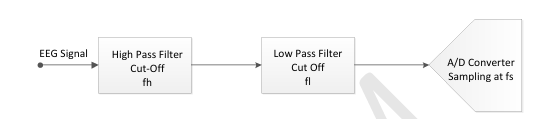
\includegraphics[width=0.8\columnwidth]{figs/Q45.png}
\label{fig:Q45.png}
\end{figure}

\hfill{\brak{\text{GATE BM 2024}}}

\begin{enumerate}
\item fh = 8 Hz, fl = 12 Hz, fs = 12 Hz 
\item fh = 4 Hz, fl = 6 Hz, fs = 24 Hz 
\item fh = 6 Hz, fl = 4 Hz, fs = 12 Hz
\item fh = 8 Hz, fl = 12 Hz, fs = 48 Hz 
\end{enumerate}  

\item In the circuit below, what is the value of $I_L$ to transfer the maximum power to load? 

\begin{figure}[H]
\centering
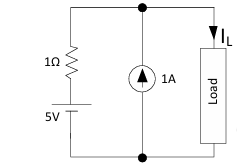
\includegraphics[width=0.5\columnwidth]{figs/Q46.png}
\label{fig:Q46.png}
\end{figure}

\hfill{\brak{\text{GATE BM 2024}}}

\begin{multicols}{4}
\begin{enumerate}
\item 3 A
\item 6 A
\item 4 A
\item 2 A
\end{enumerate}  
\end{multicols}

\item A mechanical ventilator operating in volume controlled mode is set to deliver 600mL of tidal volume (TV) with a flow rate of 40 L/min. The frequency of breathing is set  to 10 breaths per minute. If the flow rate is doubled which one of the following  happens? 

\hfill{\brak{\text{GATE BM 2024}}}

\begin{enumerate}
\item The inspiratory time will increase.
\item The expiratory time will increase.
\item The tidal volume will increase. 
\item The frequency of breathing will decrease. 
\end{enumerate}  

\item The X-ray attenuation coefficients as a function of photon energy for three materials  are shown in the figure below. A tissue phantom containing these three materials is  imaged at two different X-ray photon energies of 50 keV and 150 keV. When the 
developed X-ray film is viewed, which of the following statements is/are \textbf{TRUE}? 

\begin{figure}[H]
\centering
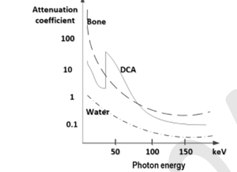
\includegraphics[width=0.5\columnwidth]{figs/Q48.png}
\label{fig:Q48.png}
\end{figure}

\hfill{\brak{\text{GATE BM 2024}}}

\begin{enumerate}
\item Bone will appear relatively brighter than DCA in 50 keV. 
\item Bone will appear relatively brighter than DCA in 50 keV. 
\item Bone will appear relatively brighter than DCA in 150 keV.
\item DCA will appear relatively brighter than bone in 150 keV. 
\end{enumerate}  

\item Which of the following is/are \textbf{TRUE} for a surface electromyography (sEMG) signal of a muscle experiencing fatigue?

\hfill{\brak{\text{GATE BM 2024}}}

\begin{enumerate}
\item The median frequency of power spectral density of sEMG will decrease. 
\item The median frequency of power spectral density of sEMG will increase. 
\item The root mean square (RMS) value of sEMG will increase. 
\item The root mean square (RMS) value of sEMG will decrease
\end{enumerate}  

\item For $\vec{F} = (x + y)\hat{i} + (x + y)\hat{j}$ the value of $\oint\vec{F}\cdot d\hat{r}$ along the path shown in the figure is \underline{\hspace{0.75cm}}. Give your answer as an integer. 

\hfill{\brak{\text{GATE BM 2024}}}

\begin{figure}[H]
\centering
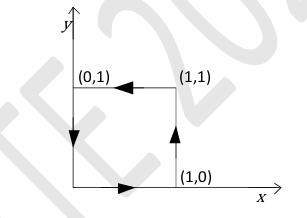
\includegraphics[width=0.5\columnwidth]{figs/Q50.png}
\label{fig:50.png}
\end{figure}

\item The approximate total cross sectional areas of various types of blood vessels are given below. It was estimated that the velocity of blood in the aorta is 30 $\text{cms}^{-1}$. The time it 
will take for the blood to travel through a capillary of length 0.5 mm is \underline{\hspace{0.75cm}} seconds. Give your answer rounded off to two decimal places.  


\begin{table}[H]
\def\arraystretch{1.5}
\centering
\begin{tabular}{|m{4cm}|m{4cm}|}
\hline
\hspace{0.75cm}vessel type & Approximation total cross sectional area ($\text{cm}^2$)\\ \hline
\hspace{1cm}Aorta&\hspace{1cm}4.5 \\ \hline
\hspace{1cm}Artery&\hspace{1cm}20 \\ \hline
\hspace{1cm}Arteriole&\hspace{1cm}400 \\ \hline
\hspace{1cm}Capillary&\hspace{1cm}4500 \\ \hline
\hspace{1cm}Venule&\hspace{1cm}40 \\ \hline
\hspace{1cm}Vein&\hspace{1cm}15 \\ \hline
\end{tabular}
\end{table}

\hfill{\brak{\text{GATE BM 2024}}}

\item A DNA extract solution with a concentration of 15 ng/$\mu$L placed in a micro-cuvette of sample thickness 0.5 mm gave an absorbance of 0.24 at a wavelength of 260 nm in a 
spectrophotometer. After further concentration, the sample was found to give an absorbance of 0.38 at the same wavelength under identical conditions. The final 
concentration of the sample is \underline{\hspace{1cm}} ng/$\mu$L. (Give your answer rounded off to 2 
decimal places.)

\hfill{\brak{\text{GATE BM 2024}}}

\item An X-ray beam of initial intensity $I_o$ of 70 keV imaging the chest is assumed to undergo 
attenuation through the muscle tissue for a thickness of 16 cm and further through the 
bone tissue for a thickness of 4 cm. The half value layer (HVL) thicknesses for the 
muscle and bone are 3.5 cm and 1.8 cm, respectively. The percentage of X-ray 
intensity transmitted through the body is \underline{\hspace{1cm}}. Give your answer rounded off to 2 
decimal places.

\hfill{\brak{\text{GATE BM 2024}}}

\item A person standing one meter away from a 4000 curie radioactive source receives a  
lethal dose of radiation in about 5 minutes. At 3 meters away from the same source, 
the time in which he will receive the same lethal dose is \underline{\hspace{1cm}}minutes. Give your 
answer rounded off to the nearest integer.

\hfill{\brak{\text{GATE BM 2024}}}

\item If a circular ultrasound transducer of radius $a$ = 8 mm operating at a central frequency 
of 1 MHz has a pressure beam pattern in a medium as given below: \\[8pt]
\begin{equation*} p(r, 0)\propto \sin \frac{ka^2}{4r}
\end{equation*}

Here, $k$ is the wave number, $r$ is the axial distance from the center of aperture. The 
speed of sound in the medium is 1600 m$\text{s}^{-1}$ \\[8pt] The reduction in intensity between $r$=8 cm and $r$=16 cm is \underline{\hspace{1cm}} dB. Give your  
answer as a positive quantity rounded off to two decimal places.

\hfill{\brak{\text{GATE BM 2024}}}

\item The source in the figure is a current source and the circuit is in steady state. At $t =$  $0.5\pi$ seconds, the value of \textbf{v} in the circuit given below is \underline{\hspace{1cm}} volts. Give your answer rounded off to 2 decimal digits.


\begin{figure}[H]
\centering
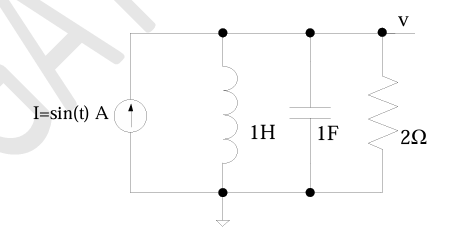
\includegraphics[width=0.6\textwidth]{figs/Q56.png}
\label{fig:Q56.png}
\end{figure}

\hfill{\brak{\text{GATE BM 2024}}}

\item The equivalent impedance, $\text{Z}_{AB}$, in the circuit given below is \underline{\hspace{1cm}} $\Omega$. Give your 
answer rounded off to one decimal place.


\begin{figure}[H]
\centering
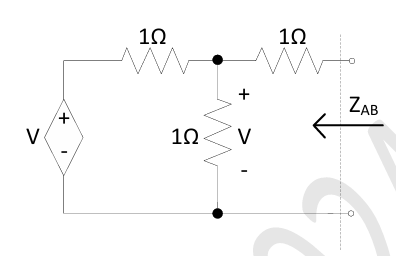
\includegraphics[width=0.6\textwidth]{figs/Q57.png}
\label{fig:Q57.png}
\end{figure}

\hfill{\brak{\text{GATE BM 2024}}}

\item The bandwidth of ECG signal ranges from 0.5 Hz to 100 Hz. If a single ADC is used to digitize data from 8 ECG channels then the minimum ADC sampling rate is \underline{\hspace{1cm}}  
Hz. Give your answer rounded off to the nearest integer.

\hfill{\brak{\text{GATE BM 2024}}}

\item If $x[n] = u[n] - u[n - 5]$, and $h[n] = \delta[n] - \delta[n - 1]$ and $y[n] = x[n] + h[n]$. then the value of $\Sigma_{n=-\infty}^{\infty}y[n]$ is \underline{\hspace{1cm}}. Give your answer rounded off to the nearest integer.

\hfill{\brak{\text{GATE BM 2024}}}

\item In the figure below, the diode is ideal. The current reading shown in the ammeter is   \underline{\hspace{1cm}} A. Give your answer rounded off to the nearest integer. 

\hfill{\brak{\text{GATE BM 2024}}}


\begin{figure}[H]
\centering
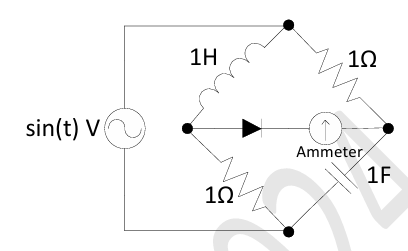
\includegraphics[width=0.6\textwidth]{figs/Q60.png}
\label{fig:Q60.png}
\end{figure}

\item In the figure below, the Fourier series of $v(t)$, in volts, is given as: \\[4pt]
\begin{equation*}
v(t) = v_o + 2\cos (\omega_ot) + \cos (5\omega_ot)
\end{equation*}
The capacitor is a short circuit for all AC signals. The power absorbed by the 1$\Omega$ resistor is \underline{\hspace{1cm}} W. Give your answer rounded off to the nearest integer. 

\begin{figure}[H]
\centering
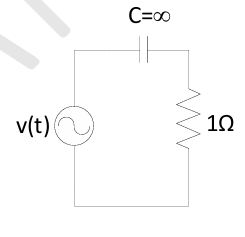
\includegraphics[width=0.5\columnwidth]{figs/Q61.png}
\label{fig:Q61.png}
\end{figure}

\hfill{\brak{\text{GATE BM 2024}}}

\item An artificial fore-arm has a moment-of-inertia around the center of mass as 0.3kg.$\text{m}^2$.  
The mass of the artificial fore-arm is 3 kg. If the distance from the elbow joint to the center of mass of the fore-arm is 20 cm, the moment-of-inertia of the fore-arm about the elbow joint is \underline{\hspace{1cm}} kg.$\text{m}^2$. Give your answer rounded off to two decimal places. 

\hfill{\brak{\text{GATE BM 2024}}}

\item A bio-potential signal of 4 mV on the skin surface was fed to an amplifier with a differential gain of 2000. The noise in the signal is 1000 mV. If the amplifier output produces a noise output of 200 mV, the common mode rejection ratio of the amplifier
is \underline{\hspace{1cm}} dB. Give your answer rounded to the nearest integer.

\hfill{\brak{\text{GATE BM 2024}}}

\item In a motor nerve conduction velocity experiment, the distance between the distal and the recording sites is 4 cm and the distance between the proximal and the recording sites is 24 cm. The distal and proximal latencies were recorded as 6 ms and 10 ms, 
respectively. The nerve conduction velocity is \underline{\hspace{1cm}} meters per second. Give your answer rounded off to the nearest integer.

\hfill{\brak{\text{GATE BM 2024}}}

\item A person creates an apparatus as shown in the figure to exercise the extensor muscle 
of the hand. It is given that OP = 0.15 m, OQ = 0.35 m, $\theta = 30^\circ$, the weight of the 
lower arm = 20 N, the center of mass of the lower arm is at point P, the magnitude of the applied tensile force F = 50 N. If the extensor muscle is acting with a moment arm of 0.25 m, the muscle force required to hold the hand at the position shown in the figure \underline{\hspace{1cm}}N. Give your answer rounded off to the nearest integer.

\hfill{\brak{\text{GATE BM 2024}}}

\begin{figure}[H]
\centering
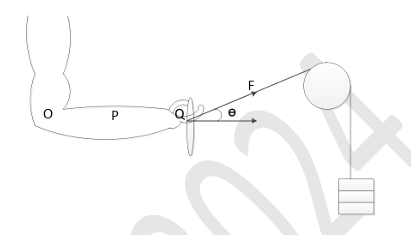
\includegraphics[width=0.6\textwidth]{figs/Q65.png}
\label{fig:Q65.png}
\end{figure}


\end{enumerate}



























































































































    
\end{document}

